% !TeX spellcheck = en_US
\section{Problem 5}

This problem relies on the parametric neural network from the previous problem, only that this time we have $S^1=12$ and learning rate $\alpha=0.1$. Despite the use of MATLAB programming language in Problem 4, this time we opted to use python-TensorFlow. It still uses all of the matrix operations that we used earlier but they are abstracted from the end user who just calls an API. The engine does the rest.\\

Looking at figure~\ref{fig:prob5_1_12_1_nodp}, we can clearly see that there's no difference between it and figure~\ref{fig:prob4_1-12-1_error_output}. This means that we're on the same level as before (\textit{same constraints, weight and bias initialization etc.}) and we can continue on this problem.
The code for this is located at \verb|Problem 5/keras_backprop.py|.\\


\begin{wrapfigure}{r}{0.45\textwidth}
	\centering
	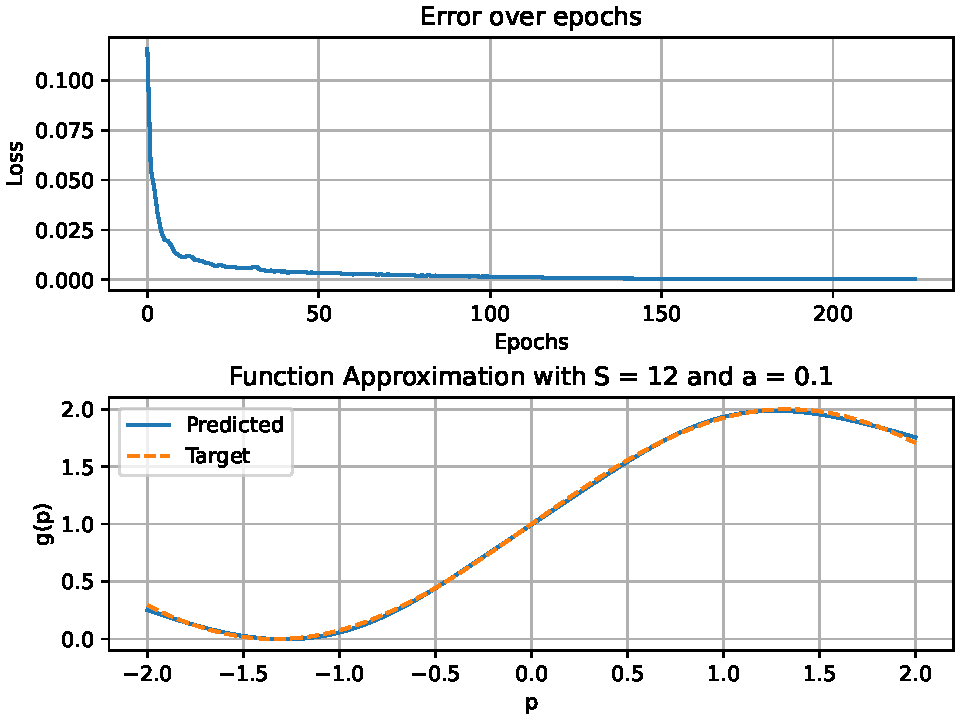
\includegraphics[width=0.43\textwidth]{../Problem 5/nn_1_12_1_nodp.pdf}
	\caption{Approximated function and error over iterations}
	\label{fig:prob5_1_12_1_nodp}
\end{wrapfigure}


In order for us to not have unnecessary computations, we implemented \verb|Early Stopping|. This is a method that stops a neural network's train if there aren't significant changes in approximation error.\\

Backdrop implementation was fairly easy. We just added the Dropout layer between the first and last layer with the appropriate probability $\theta$ every time. TensorFlow assures us that the dropout layer we just added will not be used during testing.\\
After the model's been created, we run the program and produce the images in figure complex~\ref{fig:prob5_1_12_1_all_dropout}.

We can see from the figures that, the approximation is not working at all, despite the loss function being so low. The approximated function \say{crosses} the input one 2 or 3 times at most, making the approximation a low fidelity one.
Also, the loss function over iterations jumping all over the place as epochs progresses.

\begin{figure}[htpb]
	\centering
	\begin{subfigure}{0.47\textwidth}
		\centering
		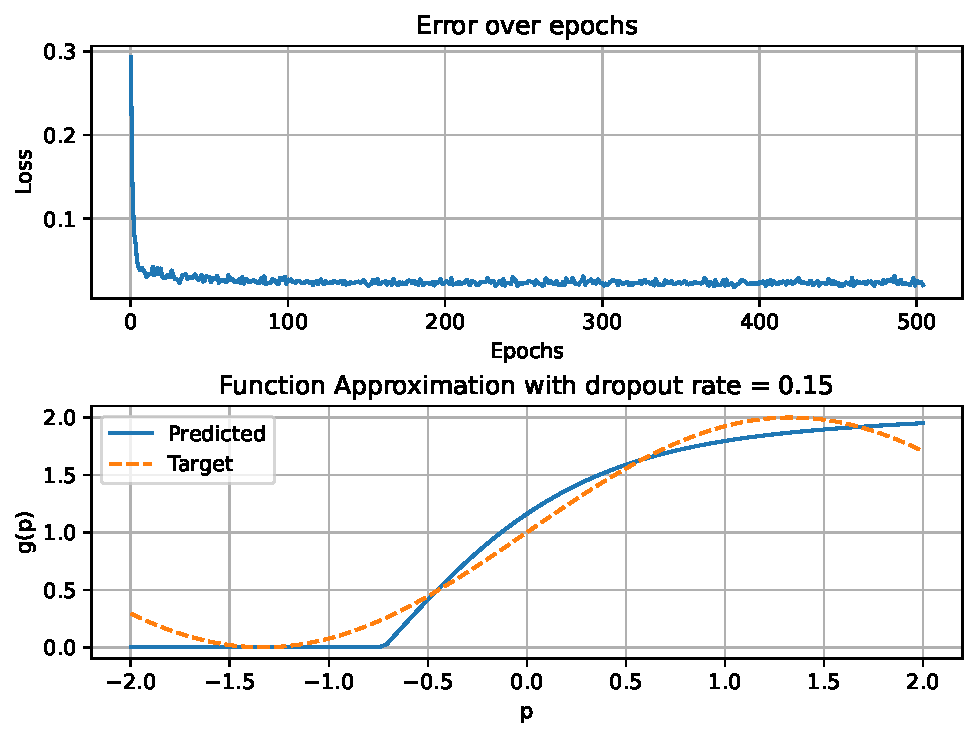
\includegraphics[width=\textwidth]{../Problem 5/nn_1_12_1_0.15.pdf}
		\caption{$\theta=0.15$}
	\end{subfigure}
	\hfill
	\begin{subfigure}{0.47\textwidth}
		\centering
		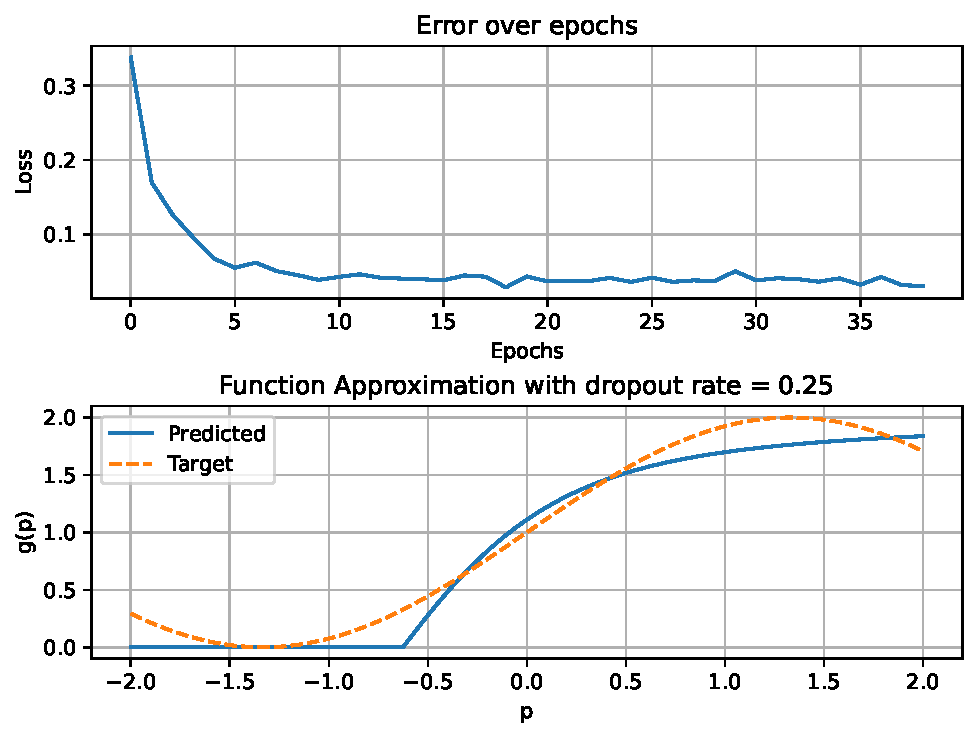
\includegraphics[width=\textwidth]{../Problem 5/nn_1_12_1_0.25.pdf}
		\caption{$\theta=0.25$}
	\end{subfigure}\\
	\vspace{1cm}
	\begin{subfigure}{0.47\textwidth}
		\centering
		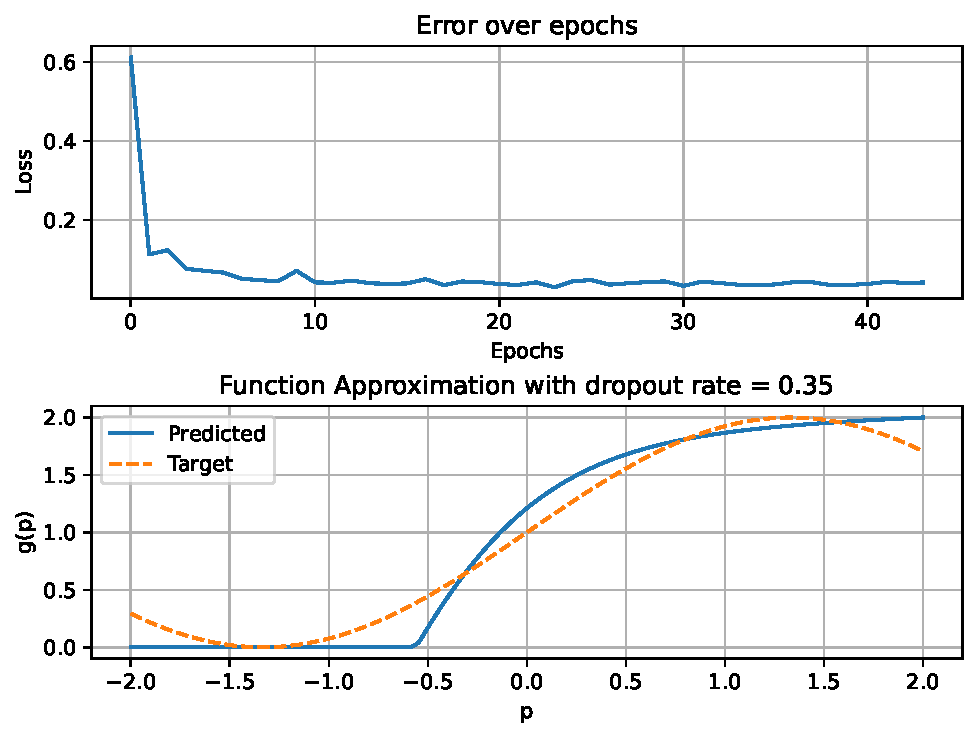
\includegraphics[width=\textwidth]{../Problem 5/nn_1_12_1_0.35.pdf}
		\caption{$\theta=0.35$}
	\end{subfigure}
	\caption{Loss and approximation of input for multiple $\theta$ values.}
	\label{fig:prob5_1_12_1_all_dropout}
\end{figure}

Specifically, for $\theta = \{0.15, 0.25\}$, the loss decreases sharply at the beginning and then plateaus, suggesting that the model is quickly learning the function but then reaches a point where additional learning is marginal.
For $\theta = 0.35$, the loss decreases more slowly, indicating that a higher dropout rate might be slowing down the learning process or improving generalization by preventing overfitting.\\

As far as the approximation of the input signal is concerned, 
for $\theta = 0.15$, the predicted function seems to fit the target quite well, except for slight deviations at the boundaries ($p = -2$ and $p = 2$).
For $\theta = 0.25$, the fit is less accurate, with noticeable divergence from the target, especially for values of p greater than 1.
Lastly, for $\theta = 0.35$, the predicted function deviates significantly from the target across almost the entire range of p, indicating that the model may be underfitting, possibly due to too much regularization from the dropout.
